\documentclass[12pt]{article}
\usepackage[T1]{fontenc}
%\usepackage[latin9]{inputenc}
\usepackage[utf8]{inputenc}
\usepackage[english]{babel}
\usepackage{amsmath}
\usepackage{amsfonts}
\usepackage{amssymb}
%\usepackage{setspace}
\usepackage{rotating}
\usepackage{graphics}
\usepackage{eurosym}
\usepackage[round]{natbib}
%\usepackage{graphicx}
%\usepackage{float} 				%allows you to float images
\usepackage{latexsym}
%\usepackage{bbding}
%\usepackage {moresize}
\usepackage{listings}
\usepackage{bbding}
\usepackage{blindtext}
\usepackage{hhline}
\usepackage{tikz}
\usetikzlibrary{trees}
%\usetikzlibrary{shapes,backgrounds}
%\usepackage{pgfplots}
%\usetikzlibrary{arrows}
\usepackage{enumitem}
%\doublespacing
%\usepackage{geometry}
\usepackage{amsthm}
\usepackage{color}
%\usepackage{array,multirow}
%\usepackage{subcaption}
%\usepackage{pst-plot}
%	\psset{xunit=15mm}
%\geometry{verbose,tmargin=1in,bmargin=1in,lmargin=.5in,rmargin=.5in}
\setlength{\parskip}{\bigskipamount}
\setlength{\parindent}{0pt}
\usepackage{multicol}

\newenvironment{problem}[3][Problem]{\begin{trivlist}
\item[\hskip \labelsep {\bfseries #1}\hskip \labelsep {\bfseries #2.}]}{\end{trivlist}}

\newcommand{\barr}{\bar{r}}
\newcommand{\ddx}{\frac{d}{dx}}
\newcommand{\infsum}{\sum_{n=1}^{\infty }}

\title{Problem Set 6 \thanks{Problems:5.2,5.4,5.6,5.7,5.12,5.16,5.17,5.20,5.27}}
\author{Ian McGroarty \\
	Course Number: 555.444 \\
Sorry this is so late professor! It has been a busy two weeks!}
\date{October 7, 2019}

\begin{document}

\maketitle
\newpage
%%%%%%%%%%%%%%%%%%%%%%%%%%%%%%%%%%%%%%%%%%%%%%%%%%%%%%%%
%%%%%%%%%%%%%%%%%%%%%%%%%%%%%%%%%%%%%%%%%%%%%%%%%%%%%%%%
%%%%%%%%%%%%%%%%%%%%%%%%%%%%%%%%%%%%%%%%%%%%%%%%%%%%%%%%
\begin{problem}{7.1}. Well A has a comparative advantage in fixed rates and B has a comparative advantage in floating rates. We see the difference as $A: 5+0.1 = 5.1$ and $B: 6.4 + 0.6 = 7.0$ so $7.0-5.1 = 1.9$ If we say that 1\% goes to the financial intermediary, and A and B evenly split the rest, $(1.9-0.1)=1.8/2=0.9$. So something like the following will occur: 
\begin{itemize}
\item A pays 5\% per annum to outside lenders. 
\item A pays LIBOR to the financial intermediary. 
\item A receives 5.9\% from the financial intermediary 
\item B pays LIBOR = 0.6\% per annum to outside lenders 
\item B pays 5.9\% to the financial intermediary 
\item B receives LIBOR from the Financial intermediary. 
\end{itemize}
The net effect for A is: $LIBOR + 5 -5.9 = LIBOR -0.9$ So it is a full 1\% better off than it would be if it it just went to the floating rate market! The net effect for B is $LIBOR +0.6 -LIBOR -5.9 = -5.3\%$ so it is 1.1\% better off than if it went straight to the fixed rate market. 

$\begin{bmatrix}
\leftarrow 5\% \leftarrow &A & \leftarrow 5.95\% \leftarrow & FI & \leftarrow 5.95\% \leftarrow & B & \\
 & A & \rightarrow LIBOR  \rightarrow & FI & \rightarrow LIBOR  \rightarrow & B & \rightarrow LIBOR + 0.6\% \\
\end{bmatrix}$
\end{problem}
\newpage


\begin{problem}{7.3}. Okay so first it is basically a 12 month made up of 6 months. So there will be a payment made and received at 6 months (in 4 months) and also at 12 months (in 10 months). We see what it will be paid (as per 6 month rate 2 months ago) in 4 months (6 months from two months ago): $0.5*0.046*100=2.3$ million. Next we will see what will be received ( as per contract): $0.5*0.07*100=3.5$ million. This amount will also be received in 10 months at the end of the contract (plus the 100 million). Discounting the amounts received the corresponding length of time; the value of the fixed rate bond is: $$3.5\cdot e^{-0.05\cdot 4/12} + 103.5\cdot e^{-0.05\cdot 10/12} = 3.44215 + 99.27= \$ 102.72 \ million$$
The value of the floating rate bond is:
$$ (100+2.3)\cdot e^{-0.05\cdot 4/12} = \$100.61 \ million$$
Thus, the value of the swap to the party paying floating: $102.72-100.61 = \$ 2.11 \ million$. For the value to be zero we must have that the value to the party paying the fixed: $\$-2.11 \ million$
\end{problem}




\begin{problem}{7.5}. The exchange interest in pounds is: $20 \cdot 0.10 = \pounds 2 \ million$. Similarly, the exchange interst in dollars is $30 \cdot 0.06 = \$ 1.8 \  million$
\end{problem}

\begin{problem}{7.6}. Explain the difference between the credit risk and the market risk in a financial contract.\\
\textbf{Def: Credit Risk}: Arises from the possibility of a default by the counterparty when the value of the contract to the financial institution is positive. \\
\textbf{Def: Market Risk}: Arises from the possibility that the market variables such as interest rates and exchange rates will move in such a way that the value of a contract to the financial institution becomes negative. 

I think that the definition does a good job of explaining the difference. It might also be important to note that market risk is hedged using financial tools whereas credit risk is hedged using a financial intermediary. However, I think that these two risks are related in that the market risk of the counterparty impacts the credit risk. That is why it is important to do things like stress testing. 
\end{problem}


\begin{problem}{7.9}. So X has the comparative advantage in the fixed rates. Te difference is 0.8\% less 0.2\% for the financial intermediary is 0.6\%/2 = 0.3\%. So if all goes well they will both benefit 0.3\%. Since A has the comparative advantage we in fiexed rate and B has the comparative advantage in floating we can do the following: 
\begin{itemize}
\item X pays 8\% per annum to outside lenders
\item X pays LIBOR to the FI
\item X receives (8+0.3=)8.3\% from FI
\item Y pays LIBOR to outside investors
\item Y pays (8.8-0.3=)8.5\% to the FI
\item Y receives LIBOR from the FI. 
\end{itemize}
The end result is that X pays (8+LIBOR -8.3) = LIBOR -0.3. This is 0.3\% better than if it went to floating by itself. Y pays (LIBOR + 8.5-LIBOR) = 8.5. This is 0.3\% better than if it went to fixed by itself. And the FI walks away with 0.2\%.

$\begin{bmatrix}
\leftarrow 8\% \leftarrow &X & \leftarrow 8.2\% \leftarrow & FI & \leftarrow 8.5\% \leftarrow & Y & \\
 & X & \rightarrow LIBOR  \rightarrow & FI & \rightarrow LIBOR  \rightarrow & X& \rightarrow LIBOR  \\
\end{bmatrix}$
\end{problem}


\begin{problem}{7.12}. The table below shows the calculations made to reach the conclusion that the cost to the fincial institution is \$680,000. \\
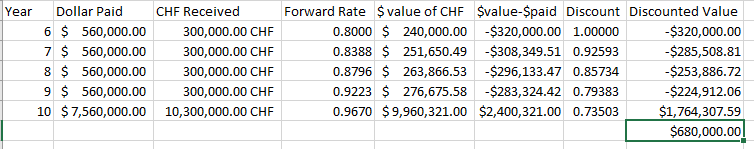
\includegraphics[width=\textwidth]{mod6_p712b.png}
\end{problem}
\newpage 
\begin{problem}{7.18}. First we need the two year zero rate. Semiannual means $5.4/2=2.7\% $ coupon payments at 0.05\% until the fourth payment which will be at the zero rate. By definition the zero rate will have to be such that: 
$$ 2.7e^{-0.05\cdot 0.5} + 2.7e^{-0.05\cdot 1}+2.7e^{-0.05\cdot 1.5} 102.7e^{R_2\cdot 2 }= 100$$
This gives us $R_2=0.5342$. A similar process can be done for 2.5 year zero rate with $(5.4+5.6)/2=5.5/2=2.75\% $ 
$$ 2.75e^{-0.05\cdot 0.5} + 2.75e^{-0.05\cdot 1}+2.75e^{-0.05\cdot 1.5} 102.75e^{R_{2.5}\cdot 2 }= 100$$
Which gives us $R_{2.5}=0.054$, it then follows that $R_3 = 0.055$.
\end{problem}

\begin{problem}{7.23}. NOTE: This version of the problem is missing the zero rate: In the book version the zero rate is 3.8 so I\rq{}ll use that? \\
14 months, means a payment was made last month (we can ignore) and a payment will be made in 2,5,8,11,14 months. We calculate the \underline{quarterly} payments to be: $100\cdot 0.1/4=\$2.5 \ million$. The agreed to receive 3 month LIBOR. In 2 months, they will receive $(100 \cdot 0.118/4) = \$ 2.95\ million$. in the remaining months (5-14) they will receive $(100 \cdot 0.12/4)=\$ 3 \ million$. To find the value all we have to do is discount and sum:
$(2.95-2.5)\cdot e^{-0.038 \cdot 2/12} + (3-2.5)\cdot e^{-0.038 \cdot 5/12} + (3-2.5)\cdot e^{-0.038 \cdot 8/12} + (3-2.5)\cdot e^{-0.038 \cdot 11/12} + (3-2.5)\cdot  e^{-0.038 \cdot 14/12} = \$2.388 \ million$
\end{problem}
\newpage
\begin{problem}{7.24}. So first note that  B as an absolute advantage in both. But A will still have a comparative advantage in sterling relative to B (since the difference is smaller so the opportunity cost for A is smaller). Next, if A is to borrow USD it will have to receive the 11\% GBP from the financial intermediary, similarly for B will have to receive 6.2\% from the financial intermediary. 

Now A can give up to \$ 7\% USD to the FI in order to break even and B can give up to \pounds 10.6\%. So at least 4 extra basis points will have to come from A so the financial intermediary can afford to give A \pounds 11\%. That means A is going to have to give at least \$ 6.6\%. The FI demands 10 basis points, so we take 5 from each, but B is already maxed out a 10.6 so we have to take all 10 from a bringing up the payment $A\rightarrow FI$ to \$ 6.7\%.  So, in this scenario A gains 30 basis points, FI gains 10, and B gains 0. So we can spread out A\rq{}s surplus to B and have the following arrangement:
\begin{itemize}
\item A pays \pounds 11 \% to outside lenders
\item A pays \$ 6.85 \% to FI
\item A receives \pounds 11\% from FI
\item B pays \$ 6.2\% to outside lenders
\item B pays \pounds 10.45\% to FI
\item B receives \$ 6.2\% from FI
\end{itemize}

$\begin{bmatrix}
\leftarrow \pounds 11 \% \leftarrow &A & \leftarrow \pounds 11 \% \leftarrow & FI & \leftarrow \pounds 10.45\% \leftarrow & B & \\
 & A & \rightarrow \$ 6.85 \%   \rightarrow & FI & \rightarrow \$ 6.2 \%   \rightarrow & B & \rightarrow \$ 6.2 \%\\
\end{bmatrix}$


\end{problem}
\end{document}



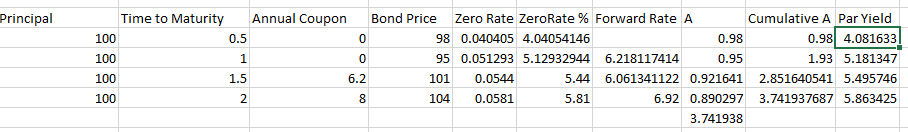
\includegraphics[width=\textwidth]{mod3_p434.png}
% Set the overall layout of the tree




\tikzstyle{level 1}=[level distance=3.5cm, sibling distance=3.5cm]
\tikzstyle{level 2}=[level distance=3.5cm, sibling distance=2cm]

% Define styles for bags and leafs
\tikzstyle{bag} = [text width=4em, text centered]
\tikzstyle{end} = [circle, minimum width=3pt,fill, inner sep=0pt]

\begin{tikzpicture}[grow=right, sloped]
\node[bag] {Bag 1 $4W, 3B$}
    child {
        node[bag] {Bag 2 $4W, 5B$}        
            child {
                node[end, label=right:
                    {$P(W_1\cap W_2)=\frac{4}{7}\cdot\frac{4}{9}$}] {}
                edge from parent
                node[above] {$W$}
                node[below]  {$\frac{4}{9}$}
            }
            child {
                node[end, label=right:
                    {$P(W_1\cap B_2)=\frac{4}{7}\cdot\frac{5}{9}$}] {}
                edge from parent
                node[above] {$B$}
                node[below]  {$\frac{5}{9}$}
            }
            edge from parent 
            node[above] {$W$}
            node[below]  {$\frac{4}{7}$}
    }
    child {
        node[bag] {Bag 2 $3W, 6B$}        
        child {
                node[end, label=right:
                    {$P(B_1\cap W_2)=\frac{3}{7}\cdot\frac{3}{9}$}] {}
                edge from parent
                node[above] {$B$}
                node[below]  {$\frac{3}{9}$}
            }
            child {
                node[end, label=right:
                    {$P(B_1\cap B_2)=\frac{3}{7}\cdot\frac{6}{9}$}] {}
                edge from parent
                node[above] {$W$}
                node[below]  {$\frac{6}{9}$}
            }
        edge from parent         
            node[above] {$B$}
            node[below]  {$\frac{3}{7}$}
    };
\end{tikzpicture}


\section{Definitions}
\underline{Def: Forward Rate Formulas} (pg 79). The implied forward rate between times $t_1$ and $t_2$ is the rate of interset between those times that is consistent with a given spot rate curve. For Yearly compounding, the forward rate is:  
\begin{align*}
f_{i,j} =& [\frac{(1+s_j)^j}{(1+s_i)^i}]^{1/(j-i)}-1 \\
 e^{s(t_2)t_2} =& e^{s(t_1)t_1}e^{f_{t_1,t_2}(t_2-t_1)}
\end{align*}

\underline{Discount Factor Relation} The discount facot between periods i and j is defined as $$ d_{i,j}=[\frac{1}{1+f_{i,j}}]^{j-i}$$ These factors satisfy the compounding rule: $d_{i,k}=d_{i,j}d_{j,k}$\\

\underline{Def. Derivative (Ross pg 223)} Let F be a real valued function defined on an open interval contained a point a. We say f is differentiable at a, or f has derivative at a if the limit $$ f'(a) = \lim_{x \to a} \frac{f(x)-f(a)}{x-a} $$




https://www.investopedia.com/university/advancedbond/bond-pricing.asp
https://quant.stackexchange.com/questions/22288/duration-of-perpetual-bond
http://people.stern.nyu.edu/gyang/foundations/sample-final-solutions.html
http://pages.stern.nyu.edu/~jcarpen0/courses/b403333/07convexh.pdf
https://web.stanford.edu/class/msande247s/2009/summer%2009%20week%205/Bond%20Formula%20Sheet.pdf


\underline{Def: Forward Rate Formulas} (pg 79). The implied forward rate between times $t_1$ and $t_2$ is the rate of interset between those times that is consistent with a given spot rate curve. For Yearly compounding, the forward rate is:  
\begin{align*}
f_{i,j} =& [\frac{(1+s_j)^j}{(1+s_i)^i}]^{1/(j-i)}-1 \\
 e^{s(t_2)t_2} =& e^{s(t_1)t_1}e^{f_{t_1,t_2}(t_2-t_1)}
\end{align*}

\underline{Discount Factor Relation} The discount facot between periods i and j is defined as $$ d_{i,j}=[\frac{1}{1+f_{i,j}}]^{j-i}$$ These factors satisfy the compounding rule: $d_{i,k}=d_{i,j}d_{j,k}$\\

\underline{Def. Derivative (Ross pg 223)} Let F be a real valued function defined on an open interval contained a point a. We say f is differentiable at a, or f has derivative at a if the limit $$ f'(a) = \lim_{x \to a} \frac{f(x)-f(a)}{x-a} $$



\begin{align*}
\text{Maximize  } & 4x_1 +5x_2 +3x_3 +4.3x_4 + x_5 + 1.5x_6 + 2.5x_7 + 0.3x_8 + x_9 + 2x_{10} \\
\text{Subject to } & 2x_1 + 3x_2 + 1.5x_3 + 2.2x_4 +0.5x_5 +15x_6 + 2.5x_7 +0.1x_8 + 0.6x_9 + x_{10} \leq 5 \\ 
& x_1 + x_2 + x_3 + x_4 \leq 1 \\
& x_5 + x_6 + x_7 \leq 1 \\
& x_8 + x_9 + x_{10} \leq 1 \\
\end{align*}